\documentclass{ximera}

%\usepackage{todonotes}

\newcommand{\todo}{}

\usepackage{tkz-euclide}
\tikzset{>=stealth} %% cool arrow head
\tikzset{shorten <>/.style={ shorten >=#1, shorten <=#1 } } %% allows shorter vectors

\usepackage{tkz-tab}  %% sign charts
\usetikzlibrary{decorations.pathreplacing} 

\usetikzlibrary{backgrounds} %% for boxes around graphs
\usetikzlibrary{shapes,positioning}  %% Clouds and stars
\usetikzlibrary{matrix} %% for matrix
\usepgfplotslibrary{polar} %% for polar plots
\usetkzobj{all}
\usepackage[makeroom]{cancel} %% for strike outs
%\usepackage{mathtools} %% for pretty underbrace % Breaks Ximera
\usepackage{multicol}

\usepackage{polynom}



\usepackage[many]{tcolorbox}  %% for titled boxes
\newtcolorbox{xbox}[1]{%
    tikznode boxed title,
    enhanced,
    arc=0mm,
    interior style={white},
    attach boxed title to top center= {yshift=-\tcboxedtitleheight/2},
    fonttitle=\bfseries,
    colbacktitle=white,coltitle=black,
    boxed title style={size=normal,colframe=white,boxrule=0pt},
    title={#1}}


\usepackage{array}
\setlength{\extrarowheight}{+.1cm}   
\newdimen\digitwidth
\settowidth\digitwidth{9}
\def\divrule#1#2{
\noalign{\moveright#1\digitwidth
\vbox{\hrule width#2\digitwidth}}}





\newcommand{\RR}{\mathbb R}
\newcommand{\R}{\mathbb R}
\newcommand{\N}{\mathbb N}
\newcommand{\Z}{\mathbb Z}

%\renewcommand{\d}{\,d\!}
\renewcommand{\d}{\mathop{}\!d}
\newcommand{\dd}[2][]{\frac{\d #1}{\d #2}}
\newcommand{\pp}[2][]{\frac{\partial #1}{\partial #2}}
\renewcommand{\l}{\ell}
\newcommand{\ddx}{\frac{d}{\d x}}
\newcommand{\ddt}{\frac{d}{\d t}}

\newcommand{\zeroOverZero}{\ensuremath{\boldsymbol{\tfrac{0}{0}}}}
\newcommand{\inftyOverInfty}{\ensuremath{\boldsymbol{\tfrac{\infty}{\infty}}}}
\newcommand{\zeroOverInfty}{\ensuremath{\boldsymbol{\tfrac{0}{\infty}}}}
\newcommand{\zeroTimesInfty}{\ensuremath{\small\boldsymbol{0\cdot \infty}}}
\newcommand{\inftyMinusInfty}{\ensuremath{\small\boldsymbol{\infty - \infty}}}
\newcommand{\oneToInfty}{\ensuremath{\boldsymbol{1^\infty}}}
\newcommand{\zeroToZero}{\ensuremath{\boldsymbol{0^0}}}
\newcommand{\inftyToZero}{\ensuremath{\boldsymbol{\infty^0}}}



\newcommand{\numOverZero}{\ensuremath{\boldsymbol{\tfrac{\#}{0}}}}
\newcommand{\dfn}{\textbf}
%\newcommand{\unit}{\,\mathrm}
\newcommand{\unit}{\mathop{}\!\mathrm}
\newcommand{\eval}[1]{\bigg[ #1 \bigg]}
\newcommand{\seq}[1]{\left( #1 \right)}
\renewcommand{\epsilon}{\varepsilon}
\renewcommand{\iff}{\Leftrightarrow}

\DeclareMathOperator{\arccot}{arccot}
\DeclareMathOperator{\arcsec}{arcsec}
\DeclareMathOperator{\arccsc}{arccsc}
\DeclareMathOperator{\si}{Si}
\DeclareMathOperator{\proj}{proj}
\DeclareMathOperator{\scal}{scal}


\newcommand{\tightoverset}[2]{% for arrow vec
  \mathop{#2}\limits^{\vbox to -.5ex{\kern-0.75ex\hbox{$#1$}\vss}}}
\newcommand{\arrowvec}[1]{\tightoverset{\scriptstyle\rightharpoonup}{#1}}
\renewcommand{\vec}{\mathbf}
\newcommand{\veci}{\vec{i}}
\newcommand{\vecj}{\vec{j}}
\newcommand{\veck}{\vec{k}}
\newcommand{\vecl}{\boldsymbol{\l}}

\newcommand{\dotp}{\bullet}
\newcommand{\cross}{\boldsymbol\times}
\newcommand{\grad}{\boldsymbol\nabla}
\newcommand{\divergence}{\grad\dotp}
\newcommand{\curl}{\grad\cross}
%\DeclareMathOperator{\divergence}{divergence}
%\DeclareMathOperator{\curl}[1]{\grad\cross #1}


\colorlet{textColor}{black} 
\colorlet{background}{white}
\colorlet{penColor}{blue!50!black} % Color of a curve in a plot
\colorlet{penColor2}{red!50!black}% Color of a curve in a plot
\colorlet{penColor3}{red!50!blue} % Color of a curve in a plot
\colorlet{penColor4}{green!50!black} % Color of a curve in a plot
\colorlet{penColor5}{orange!80!black} % Color of a curve in a plot
\colorlet{fill1}{penColor!20} % Color of fill in a plot
\colorlet{fill2}{penColor2!20} % Color of fill in a plot
\colorlet{fillp}{fill1} % Color of positive area
\colorlet{filln}{penColor2!20} % Color of negative area
\colorlet{fill3}{penColor3!20} % Fill
\colorlet{fill4}{penColor4!20} % Fill
\colorlet{fill5}{penColor5!20} % Fill
\colorlet{gridColor}{gray!50} % Color of grid in a plot

\newcommand{\surfaceColor}{violet}
\newcommand{\surfaceColorTwo}{redyellow}
\newcommand{\sliceColor}{greenyellow}




\pgfmathdeclarefunction{gauss}{2}{% gives gaussian
  \pgfmathparse{1/(#2*sqrt(2*pi))*exp(-((x-#1)^2)/(2*#2^2))}%
}


%%%%%%%%%%%%%
%% Vectors
%%%%%%%%%%%%%

%% Simple horiz vectors
\renewcommand{\vector}[1]{\left\langle #1\right\rangle}


%% %% Complex Horiz Vectors with angle brackets
%% \makeatletter
%% \renewcommand{\vector}[2][ , ]{\left\langle%
%%   \def\nextitem{\def\nextitem{#1}}%
%%   \@for \el:=#2\do{\nextitem\el}\right\rangle%
%% }
%% \makeatother

%% %% Vertical Vectors
%% \def\vector#1{\begin{bmatrix}\vecListA#1,,\end{bmatrix}}
%% \def\vecListA#1,{\if,#1,\else #1\cr \expandafter \vecListA \fi}

%%%%%%%%%%%%%
%% End of vectors
%%%%%%%%%%%%%

%\newcommand{\fullwidth}{}
%\newcommand{\normalwidth}{}



%% makes a snazzy t-chart for evaluating functions
%\newenvironment{tchart}{\rowcolors{2}{}{background!90!textColor}\array}{\endarray}

%%This is to help with formatting on future title pages.
\newenvironment{sectionOutcomes}{}{} 



%% Flowchart stuff
%\tikzstyle{startstop} = [rectangle, rounded corners, minimum width=3cm, minimum height=1cm,text centered, draw=black]
%\tikzstyle{question} = [rectangle, minimum width=3cm, minimum height=1cm, text centered, draw=black]
%\tikzstyle{decision} = [trapezium, trapezium left angle=70, trapezium right angle=110, minimum width=3cm, minimum height=1cm, text centered, draw=black]
%\tikzstyle{question} = [rectangle, rounded corners, minimum width=3cm, minimum height=1cm,text centered, draw=black]
%\tikzstyle{process} = [rectangle, minimum width=3cm, minimum height=1cm, text centered, draw=black]
%\tikzstyle{decision} = [trapezium, trapezium left angle=70, trapezium right angle=110, minimum width=3cm, minimum height=1cm, text centered, draw=black]


\outcome{Compute limits of families of functions.} 
\outcome{Compute average velocity.}
\outcome{Approximate instantaneous velocity.}
\outcome{Compare average and instantaneous velocity.}
\outcome{Plot difference quotients for varying approximations of the instantaneous rate of change.}

\title[Dig-In:]{Instantaneous velocity}

\begin{document}
\begin{abstract}
We use limits to compute instantaneous velocity.
\end{abstract}
\maketitle

When we compute average velocity, we look at 
\[
\frac{\text{change in position}}{\text{change in time}}.
\]
To obtain the (instantaneous) velocity, we want the change in time to
``go to'' zero. By this point we should know that ``go to'' is a
buzz-word for a \emph{limit}. The change in time is often given as
the length of a time interval, and this length goes to zero.

The average velocity on the (time) interval $[a,b]$ is given by
\[
v_{\text{av}} = 
\frac{\text{change in position}}{\text{change in time}} =
\frac{s(b)-s(a)}{b-a}.
\]
Here $s(t)$ denotes the position, at the time $t$, of an object moving along a line.

Let's put all of this together by working an example.

\begin{example}
A young mathematician throws a ball straight into the air with 
a velocity of 40ft/sec. Its height (in feet) after $t$ seconds 
is given by
\[
s(t) = 40t-16t^2 \qquad\text{(feet above the ground)} .
\]
Here is the graph of $s$.
\begin{image}
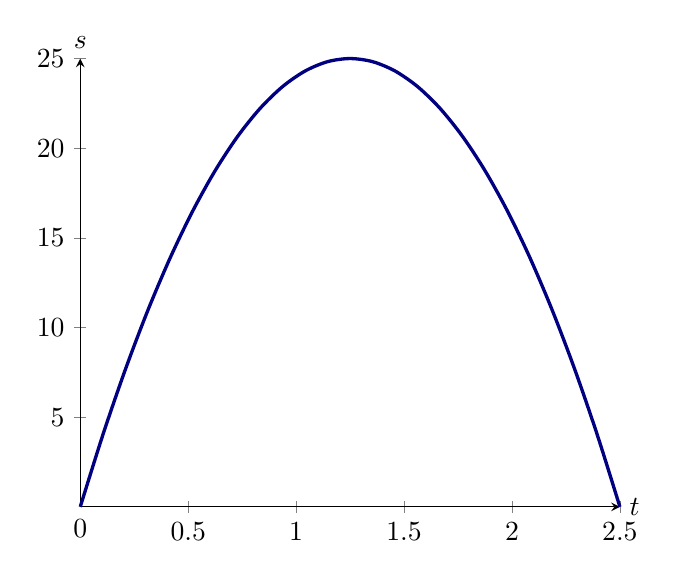
\begin{tikzpicture}
	\begin{axis}[
            clip=false, domain=0:2.5, axis lines =middle, xlabel=$t$,
            ylabel=$s$, every axis y label/.style={at=(current
              axis.above origin),anchor=south}, every axis x
            label/.style={at=(current axis.right of
              origin),anchor=west}, ]
          \addplot [very thick, penColor,smooth] {-16*x^2 +40*x};
          %\addplot [very thick,penColor2] {80};
          % \addplot [very thick,penColor4] {20};
           \node at (axis cs:0,-1.2) {$0$};
        \end{axis}
\end{tikzpicture}
\end{image}
\begin{question}
When will the ball hit the ground?

\begin{explanation}
To determine when the ball hits the ground we need to solve the
equation
\[
s(t)=0
\]
for t.  That is,
\begin{align*}
40t-16t^2 &= 0\\
t(40-16t) &= 0.
\end{align*}
This  equation has two solutions, one of them is $t=0$
seconds.
 
   Since the ball hits
the ground  some time after it's
thrown, we conclude that the ball hits the ground at time when $t>0$.
\end{explanation}
The ball will hit ground at the time
\[
t=\answer[given]{2.5}seconds.
\]

\end{question}
\begin{question}
What is the height of the ball after $2$ seconds?

\begin{explanation}
In order to find the height of the ball after $2$ seconds, we simply need 
to plug $2$ into the equation for $s(t)$.
\end{explanation} 
The height of the ball after $2$ seconds is
\[
s(2) = 40\cdot\answer[given]{2} - 16\cdot\answer[given]{2}^2 = 
\answer[given]{16}\unit{ft.}
\]

\end{question}

 Consider the following points lying along the $s$ axis.
\begin{image}
\begin{tikzpicture}
    \begin{axis}[
        ymin=-10.3,ymax=25.3,xmin=-20,xmax=20,
        clip=false,
        unit vector ratio*=1 1 1,
        axis lines=center,
        ytick={-10,-5,...,25},
        hide x axis,
        ylabel=$s$,
        every axis y label/.style={
          at={(ticklabel* cs:1)},
          anchor=south},
      ]
        \addplot[only marks,very thick,penColor,mark=*]
	        coordinates{(0,-6)};
	    \node at (axis cs:0,-6) [right] {$A$};
	    
        \addplot[only marks,very thick,penColor,mark=*]
	        coordinates{(0,0)};
	    \node at (axis cs:0,0) [right] {$B$};
	      \node at (axis cs:0,0) [left] {$0$};
	    \addplot[only marks,very thick,penColor,mark=*]
	        coordinates{(0,40-16)};
	    \node at (axis cs:0,40-16) [right] {$D$};
	    
        \addplot[only marks,very thick,penColor,mark=*]
	        coordinates{(0,40*2-16*2^2)};
	        \node at (axis cs:0,40*2-16*2^2) [right] {$C$};
        \addplot[only marks,very thick,white,mark=*]
	coordinates{(19,0)};
        \addplot[only marks,very thick,white,mark=*]
	        coordinates{(-19,0)};
    \end{axis}`
\end{tikzpicture}
\end{image}
\begin {question}
 Which points correspond to the height of the ball at time $t=0$, $t=1$ and $t=2$  seconds? 
Make  correct choices!

\begin{enumerate}
\item The point that corresponds to $s(0)$, the position (height) of the 
ball at $t=0$, is 
\begin{multipleChoice} 
\choice{A}
\choice[correct]{B}
\choice{C}
\choice{D}
\end{multipleChoice} 
\item The point that corresponds to $s(1)$, the position (height) of the 
ball at $t=1$, is 
\begin{multipleChoice} 
\choice{A}
\choice{B}
\choice{C}
\choice[correct]{D}
\end{multipleChoice} 


\item The point that corresponds to $s(2)$, the position (height) of the 
ball at $t=2$, is 
\begin{multipleChoice} 
\choice{A}
\choice{B}
\choice[correct]{C}
\choice{D}
\end{multipleChoice} 
\end{enumerate}
\end {question}

Next let's consider the average velocity of the ball.
\begin{question}
 What is the average velocity of the ball on the time interval $[1,2]$?


\begin{explanation}
In order to find the average velocity of the ball on the 
interval $[1,2]$ we recall that the average velocity on 
the time interval $[a,b]$ is given by
\[
v_{\text{av}} = 
\frac{s(b) - s\left({a}\right)}
{b-a}.
\]
Now we just plug in $a=1$ and $b=2$. 
\end{explanation}
\[
v_{\text{av}} = \frac{s(2)-s(1)}{2-1} = 
\frac{\answer[given]{16} - \answer[given]{24}}{1} =
\answer[given]{-8}\unit{ft}/\unit{s}.
\] 

Check the figure below.
\begin{image}
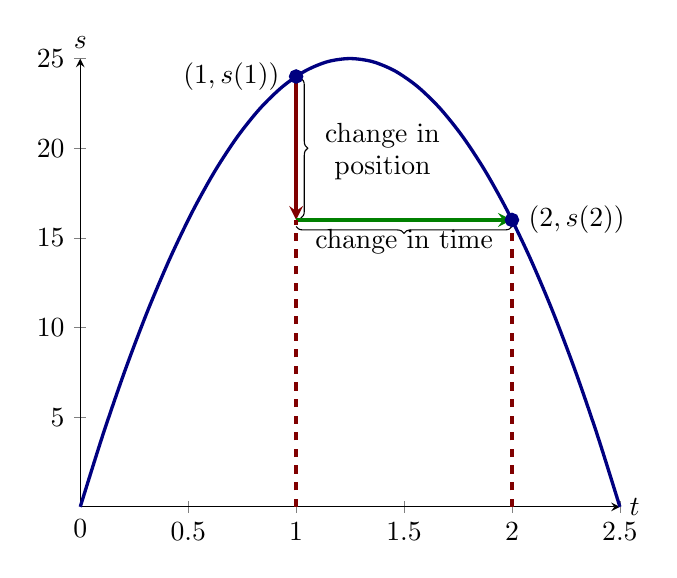
\begin{tikzpicture}
	\begin{axis}[
            clip=false, domain=0:2.5, axis lines =middle, xlabel=$t$,
            ylabel=$s$, every axis y label/.style={at=(current
              axis.above origin),anchor=south}, every axis x
            label/.style={at=(current axis.right of
              origin),anchor=west}, ]
          \addplot [very thick, penColor,smooth] {-16*x^2 +40*x};
      
       \addplot[decoration={brace,mirror,raise=.06cm},decorate,thin] plot coordinates
                       {(1,16.1) (1,23.9)};
                         \addplot[decoration={brace,mirror,raise=.06cm},decorate,thin] plot coordinates
                       {(1,15.9) (2,15.9)};
           \node at (axis cs:0,-1.2) {$0$};
             \addplot [very thick,penColor2,<-]  plot coordinates {(1,16) (1,24)};
             \addplot [very thick,penColor4,->]  plot coordinates {(1,16) (2,16)};
              \addplot [very thick,penColor2, dashed]  plot coordinates {(1,0) (1,16)};
               \addplot[only marks,very thick,penColor,mark=*]
	        coordinates{(1,24)};
	        \addplot[only marks,very thick,penColor,mark=*]
	        coordinates{(2,16)};
              % \addplot [very thick,penColor2]  plot coordinates {(1,16) (1,24)};
              \addplot [very thick,penColor2, dashed]  plot coordinates {(2,0) (2,16)};
               \node at (axis cs:1.5,14.8) {change in time};
                \node at (axis cs:1.4,20.7) {change in };
                \node at (axis cs:1.4,18.9) {position };
                 \node at (axis cs:2.3,16) {$(2,s(2))$ };
                  \node at (axis cs:0.7,24) {$(1,s(1))$ };

        \end{axis}
\end{tikzpicture}
\end{image}

\end{question}
\begin{question}
 What is the average velocity of the ball on the time interval
$[t,2]$, for $0<t<2$? 


\begin{explanation}
We use the  formula for average velocity .
\begin{align*}
v_{\text{av}} &= 
\frac{s(2)-s\left({t}\right)}
{{2}-{t}}\\
&= \frac{16 - (40t-16t^2)}{2-t}\\
&= \frac{8(2t^2-5t+2)}{2-t}\\
&= \frac{8(2t-1)\cancel{(t-2)}}{-\cancel{(t-2)}}\\
&= -8(2t-1)\\
&= 8-16t \hspace{0.06in}\unit{ft}/\unit{s},
\end{align*}
for $0<t<2$.
Check the figure below.
\begin{image}
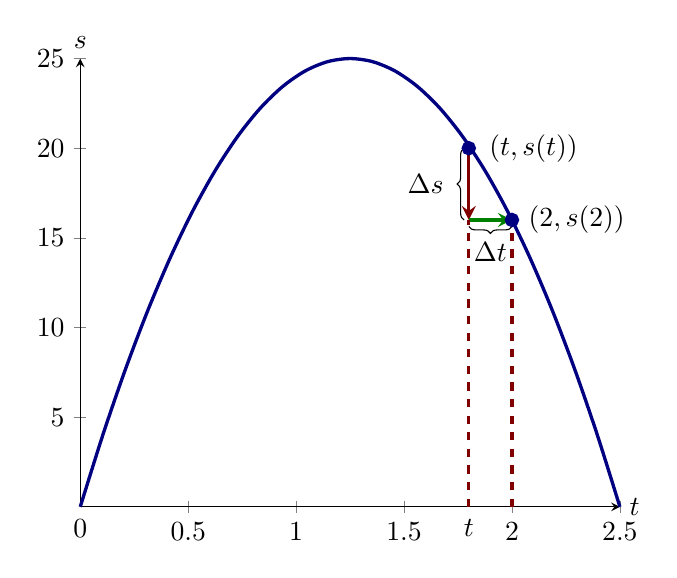
\begin{tikzpicture}
	\begin{axis}[
            clip=false, domain=0:2.5, axis lines =middle, xlabel=$t$,
            ylabel=$s$, every axis y label/.style={at=(current
              axis.above origin),anchor=south}, every axis x
            label/.style={at=(current axis.right of
              origin),anchor=west}, ]
          \addplot [very thick, penColor,smooth] {-16*x^2 +40*x};
      
       \addplot[decoration={brace,raise=.06cm},decorate,thin] plot coordinates
                       {(1.8,16) (1.8,20)};
                         \addplot[decoration={brace,mirror,raise=.06cm},decorate,thin] plot coordinates
                       {(1.8,15.9) (2,15.9)};
           \node at (axis cs:0,-1.2) {$0$};
             \addplot [very thick,penColor2,<-]  plot coordinates {(1.8,16) (1.8,20)};
             \addplot [very thick,penColor4,->]  plot coordinates {(1.8,16) (2,16)};
              \addplot [very thick,penColor2, dashed]  plot coordinates {(1.8,0) (1.8,16)};
               \addplot[only marks,very thick,penColor,mark=*]
	        coordinates{(1.8,20)};
	        \addplot[only marks,very thick,penColor,mark=*]
	        coordinates{(2,16)};
              % \addplot [very thick,penColor2]  plot coordinates {(1,16) (1,24)};
              \addplot [very thick,penColor2, dashed]  plot coordinates {(2,0) (2,16)};
               \node at (axis cs:1.9,14.2) {$\Delta t$ };
              
                \node at (axis cs:1.6,18) {$\Delta s$ };
               \node at (axis cs:1.8,-1.2) {$t$ };
                 \node at (axis cs:2.3,16) {$(2,s(2))$ };
                  \node at (axis cs:2.1,20) {$(t,s(t))$ };

        \end{axis}
\end{tikzpicture}
\end{image}
\end{explanation}
\end{question}
\begin{question}
 What is the average velocity of the ball on the interval $[2,t]$, for
$2<t<2.5$?

\begin {explanation}

The average velocity on the interval $[2,t]$, for 
$2<t<2.5$ is 
\[
v_{\text{av}} = \frac{s(t)-s(2)}{t-2} = \frac{s(2)-s(t)}{2-t}. 
\]
Notice that this is exactly the same expression we got when calculating
the average velocity on the interval $[t,2]$ for $0<t<2$. 
\end{explanation}

The average velocity on the interval $[2,t]$, for $2<t<2.5$, is given by
\[
v_{\text{av}} =\answer[given]{8-16t}\hspace{0.06in}\unit{ft}/\unit{s}.
\]

\end{question}
\begin {question}
 Using the results in Questions 5 and 6,  compute the average velocity on the interval
\begin{enumerate}
\item $[2, 2.1]$
\[
v_{\text{av}} =  8-16(\answer[given]{2.1})=-25.6 \hspace{0.06in}\unit{ft}/\unit{s}
\]
\item $[1.9,2]$
\[
v_{\text{av}} =  8-16(\answer[given]{1.9})=-22.4 \hspace{0.06in}\unit{ft}/\unit{s}
\]
\end{enumerate}
\end{question}
\end{example}

In our previous example, we computed \textit{average velocity} on
several different intervals.

 For example, the average velocity on the time interval  $[2,t]$ is  $v_{\text{av}}=8-16t$.
 
Note that the size or the length of that time interval is $t-2$.

 If we let $t\to 2$, the size of the interval will go to $0$.
 
  So, as $t$ approaches $2$,  we are computing the average velocity on smaller and
  
   smaller time intervals, and the limit of these average velocities  should be called 
 

    the \dfn{instantaneous velocity} at $t=2$.
 
 
  Limits will allow us to compute instantaneous velocity.
  
    Let's use the same setting as before.


\begin{example}
The height of a ball above the ground during the time interval  $[0,2.5]$, with $t$ is in seconds and $s(t)$ in feet, 
is given by
\[
s(t) = 40t - 16t^2.
\] 
Find $v(2)$, the instantaneous velocity of the ball $2$ seconds after it
is thrown.

\begin{explanation}
From the previous example, we know that the average velocity of the
ball on the interval $[t,2]$, for $0<t<2$, and the average velocity
on the interval $[2,t]$, for $2<t<2.5$, are both given by
\[
v_{\text{av}} =  \frac{s(t)-s(2)}{t-2}= 8-16t \hspace{0.06in}\unit{ft}/\unit{s}.
\]
In order to find the instantaneous velocity $v(2)$, we 
take the limit as $t$ goes to $\answer[given]{2}$. 
\begin{align*}
v (2)= \lim_{t\to2}v_{\text{av}}
=\lim_{t\to2}  \frac{s(t)-s(2)}{t-2}
&= \lim_{t\to2}(8-16t)\\
&= \answer[given]{-24}\unit{ft}/\unit{s}.
\end{align*}
\end{explanation}
\end{example}
\end{document}
